%%%%%%%%%%%%%%%%%%%%%%%%%%%%%%%%%%%%%%%%%%%%%%%%%%%%%%%%%%%%%%%%%%%%%%%%%%%%%%%%
% experiment.tex: Chapter describing the experiment
%%%%%%%%%%%%%%%%%%%%%%%%%%%%%%%%%%%%%%%%%%%%%%%%%%%%%%%%%%%%%%%%%%%%%%%%%%%%%%%%
%!TEX root = ../thesis_master.tex 
\chapter{The CMS Experiment}
\label{experiment_chapter}

\begin{chapquote}{Adam Lee, writing about the LHC\cite{LHCCathedial}}
``When I read that, I was reminded of the medieval cathedral builders – the architects who embarked on these grand projects knowing, or so the story goes, that they wouldn't’t see them to completion in their own lifetime. This selfless labor produced some magnificent architecture – but while I admire the beauty of great cathedrals, ultimately they’re sterile; they produce nothing of tangible benefit to humanity. But the same is not true of the great modern scientific experiments, the cathedrals of our time. These grand projects, while built on the same soaring scale and evoking the same reactions of awe and wonder, prove their worth by producing knowledge that expands our vision of the cosmos and humanity’s own place in it."
\end{chapquote}%https://www.patheos.com/blogs/daylightatheism/2010/02/cathedrals/

\section{The Large Hadron Collider}
The Large Hadron Collider (LHC) is a circular proton-proton accelerator that lies on the border between France and Switzerland \cite{LHC_DesignReport}. The ring has a circumference of 27~km and is designed to accelerate two beams of protons to a center of mass energy up to 14~TeV in order to allow the study of interactions that require a high energy scale. The LHC was commissioned in 2008, and first produced proton-proton collisions in 2009. Initially, the collider was limited to a center of mass energy of 7~TeV due to concerns over magnet stability. Over time the beam energy has been increased - first to 8~TeV in 2012, from which this data is taken, followed by 13~TeV in 2015. Luminosity has also been increasing, as can be seen in Fig \ref{fig:CMSLum}, which increases the rate of production of all interactions. The LHC is currently the highest energy accelerator in existence.
\begin{figure}[!htbp]
    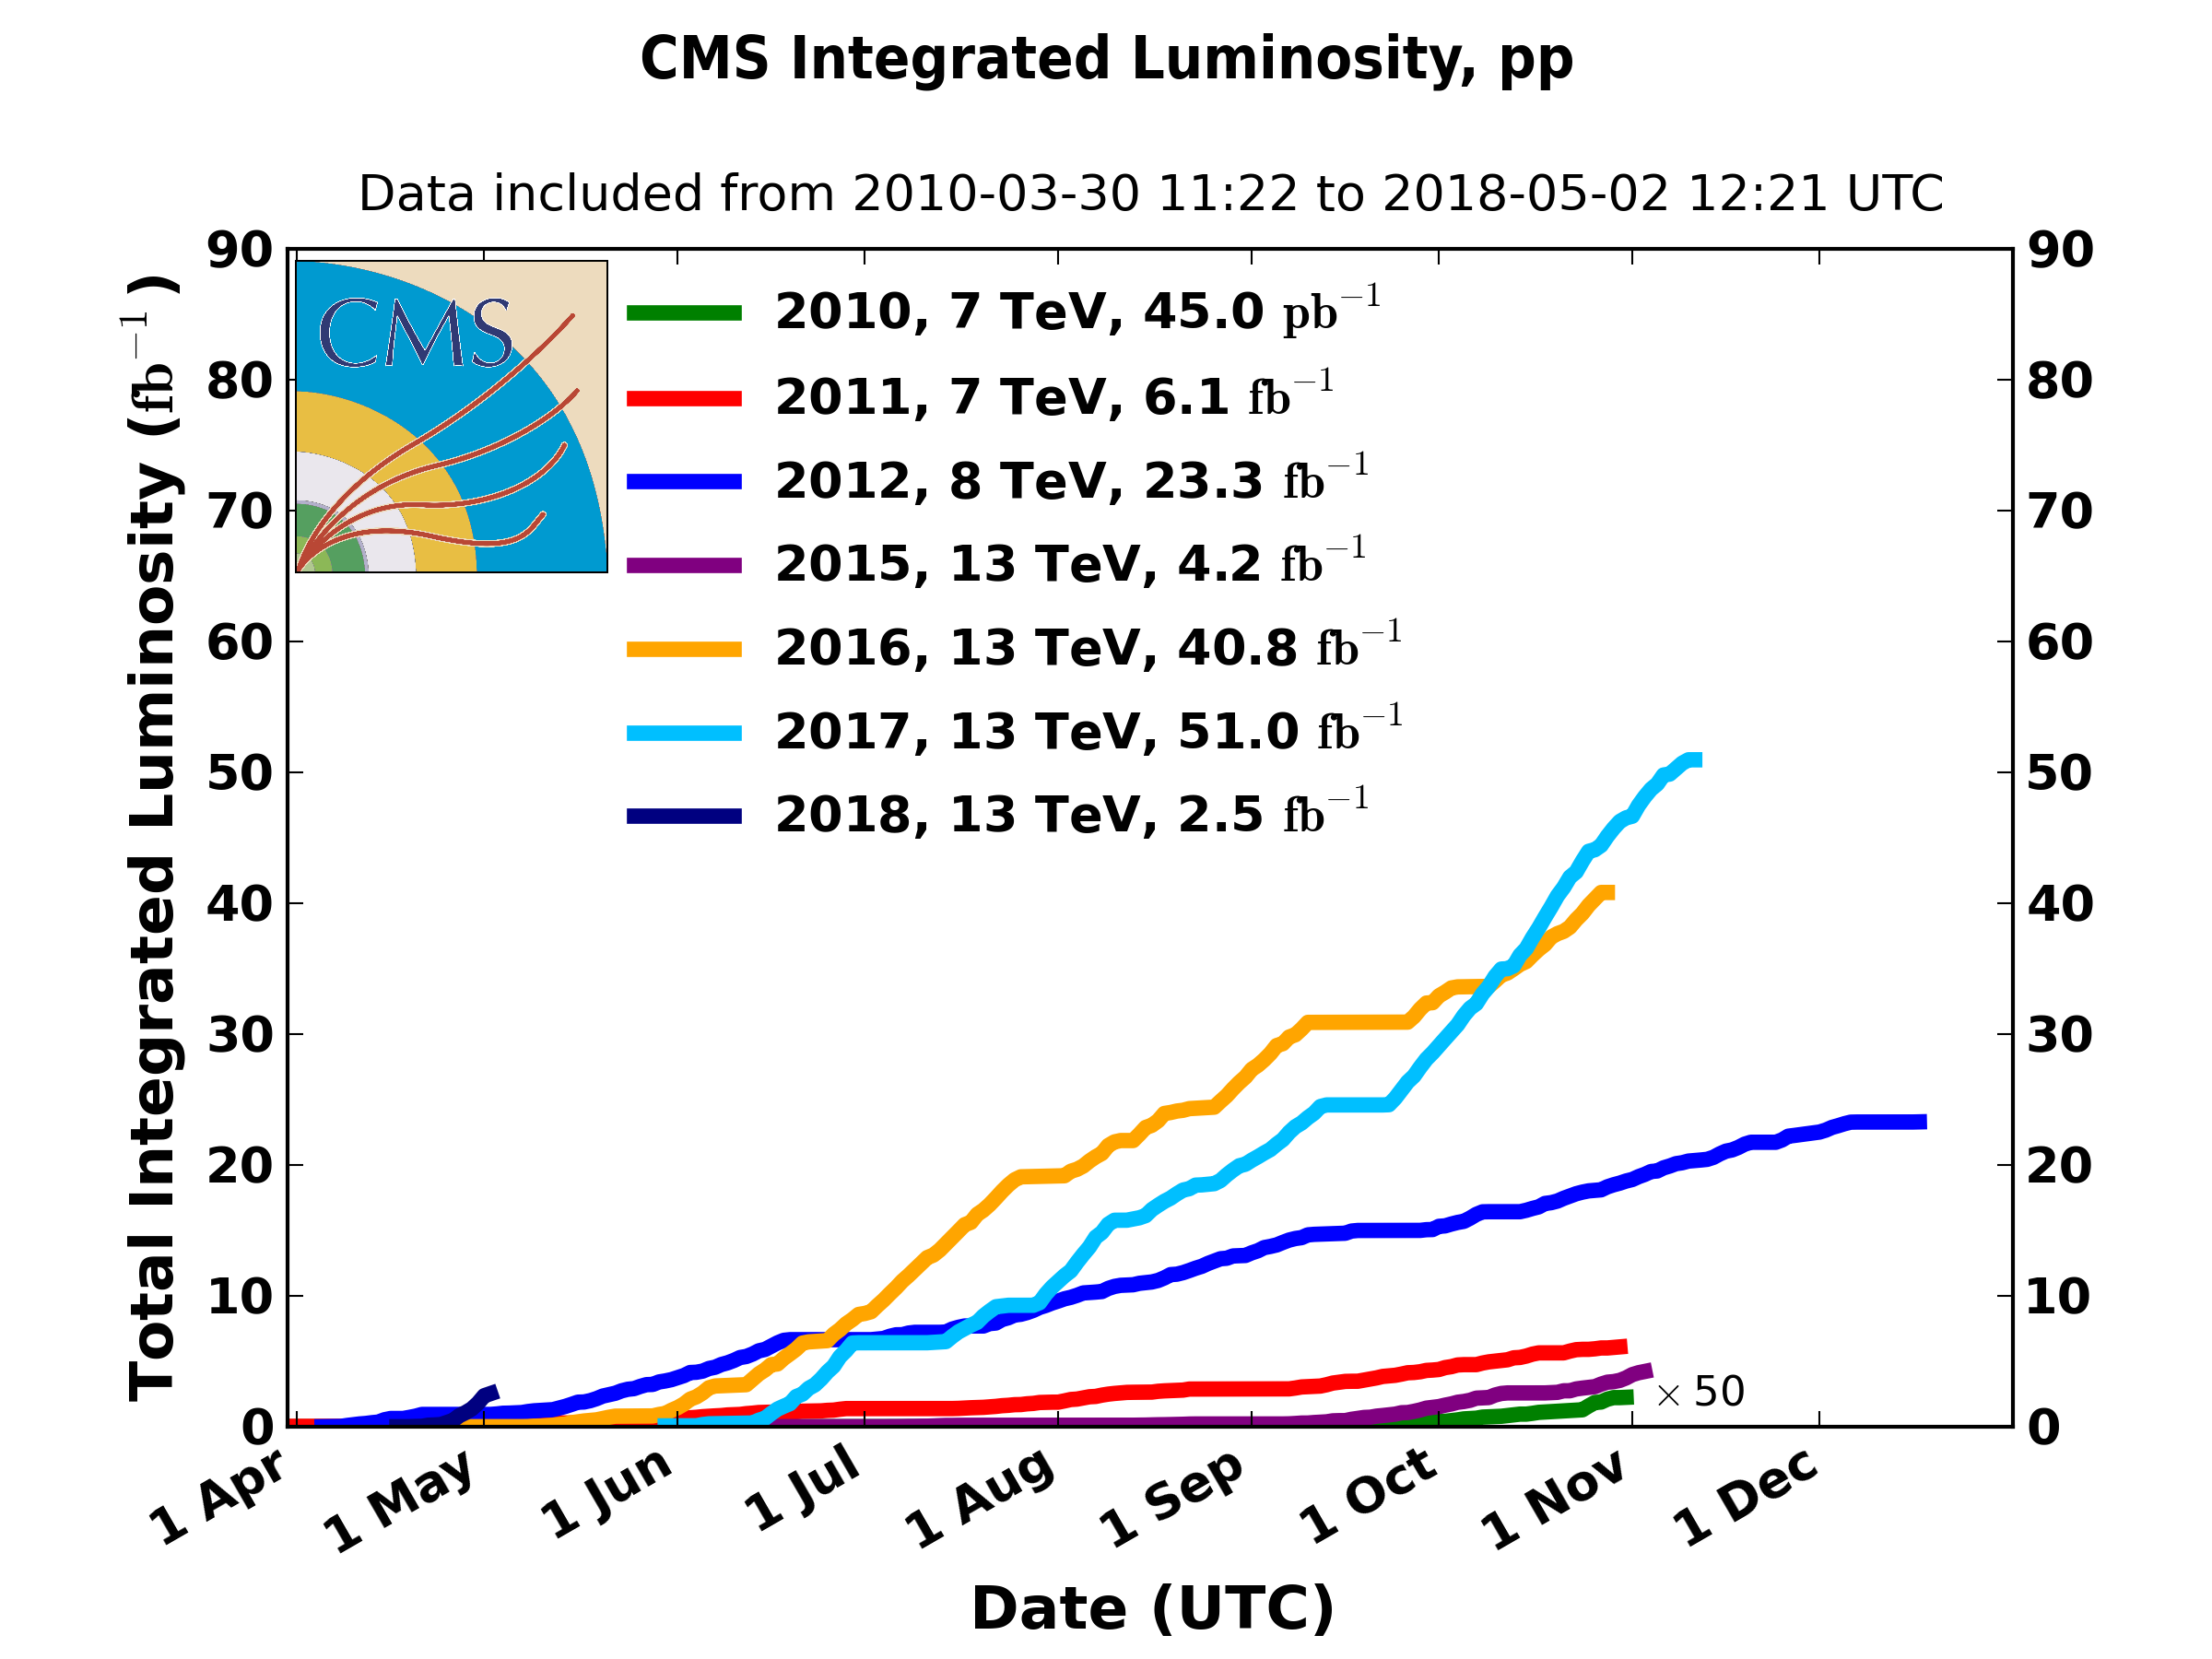
\includegraphics[width=\textwidth]{figures/ExperimentFigures/int_lumi_cumulative_pp_2.png}
    \caption[
      Luminosity seen by CMS
    ]{Comparison of luminosity of the detector. The luminosity has increased dramatically over the years.}
    \label{fig:CMSLum}
    
\end{figure}

\section{The Compact Muon Solenoid}
The Compact Muon Solenoid(CMS) detector is one of two general-purpose detectors at the LHC, and was designed to make precise measurements of the Standard Model and search for new physics. In order to accomplish this goal, CMS was built to get accurate measurements of interactions by identifying and measuring the particles produced in collisions. These measurements allow the separation of events by the type of interaction which occurred, and then each data analysis selects a particular type of interaction as `signal' and the others as `background.'
The CMS detector is made of four major sub-detectors(the tracker, the electron calorimeter, the hadron calorimeter, and the muon chambers) arranged inside or around the large solenoid for which CMS was named. This solenoid creates a magnetic field of over 3.8T, requiring a current of 20,000 A. The energy of the field is the same as half a tonne of TNT. This large field is required to get accurate measurements of charged particles momentum  using the tracker. The entire detector weighs 14,000-tonne, or as much as 80 full-grown blue whales.

In hadron collider experiments, the angular coordinate from the beam axis, which would be labeled as $\theta$ in standard polar coordinates, is instead measured using pseudorapidity $\eta$. Pseudorapidity is defined as:
\begin{equation}\label{eq:pseudorapidity}
    \eta
    =
    -\ln \Big(\tan \Big(\frac{\theta}{2}\Big)\Big).
\end{equation}
   Figure \ref{fig:mPseuodo} shows a number of different pseudorapidity values and how they relate to the beam angle.
   \begin{figure}
       \centering
       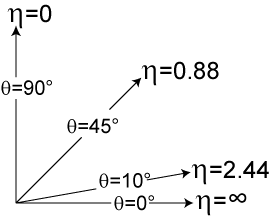
\includegraphics{figures/ExperimentFigures/Pseudorapidity2.png}
       \caption[Pseudorapidity relationship to $\theta$]{Pseudorapidity relationship to $\theta$. As can be seen, although  $\eta$ approaches infinity at $\theta=0$, $|\eta|<2.44$ contains the vast majority of the phase space for a spherically-uniform interaction. }
       \label{fig:mPseuodo}
   \end{figure}
   The use of $\eta$ is motivated by its relationship with rapidity, with $\eta\approx \rapidity$ for highly relativistic particles. Due to the kinematics of hadron colliders where the 
$z$-momentum of the collision is not fixed, many processes have a uniform rate over a significant range of \rapidity. Examples include particles in soft collisions, Fig \ref{fig:pseudorapidityDistribution}, as well as Z boson production, Fig \ref{fig:RapidityDistribution}
\begin{figure}[!htbp]
    \centering
    \begin{subfigure}[b]{0.99\SideBySidePlotWidth}
    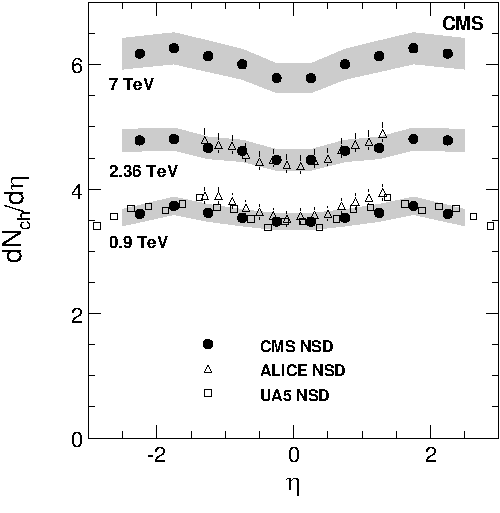
\includegraphics[width=\textwidth]{figures/ExperimentFigures/HadronPseudoRapidityDistribution.pdf}
    \caption{}
     \label{fig:pseudorapidityDistribution}
    \end{subfigure}
    \begin{subfigure}[b]{0.99\SideBySidePlotWidth}
        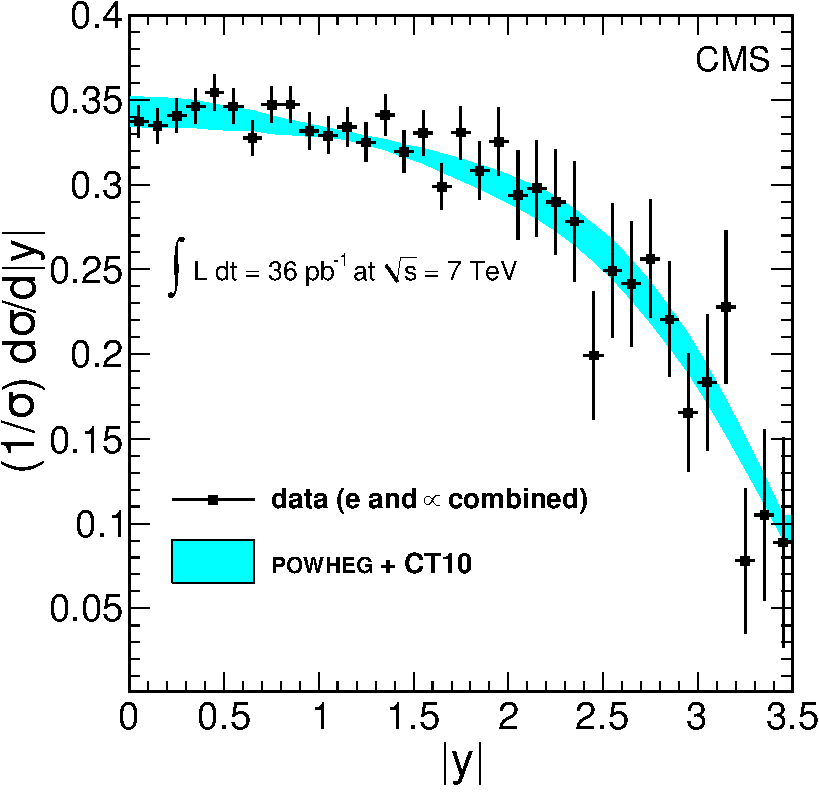
\includegraphics[width=\textwidth]{figures/ExperimentFigures/ZRapidityDistributionPlot.pdf}
        \caption{}
         \label{fig:RapidityDistribution}
     \end{subfigure}
    \caption{Two plots showing similarities between rapidity distributions and pseudorapidity.  The left plot shows the distribution of pseudorapidity for charged hadrons in underlying events at multiple center of mass energies \cite{Khachatryan:2010us}. The right plot shows the rapidity distribution of Z bosons at CMS at 7 TeV \cite{Chatrchyan:2011wt}. As can be seen from the plots both particle rates relatively constant over a wide range of \rapidity and $\eta$ with a cutoff inversely related mass of the particle, with the cutoff for the Z being smaller than for the pions for the underlying event)}
    \label{fig:RapidityandPseudorapidityDistribution}
\end{figure}

\begin{figure}[!htbp]
    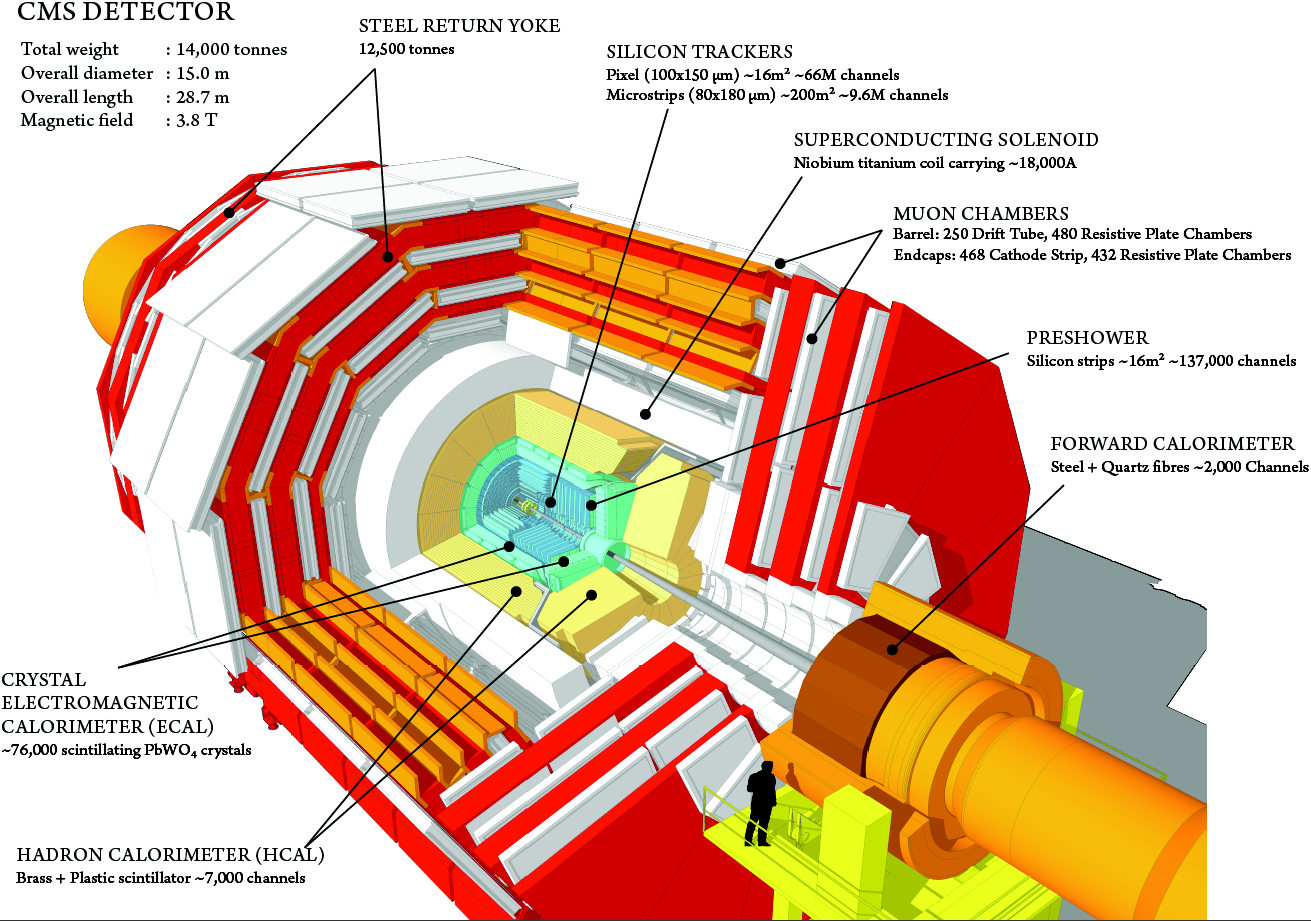
\includegraphics[width=\textwidth]{figures/ExperimentFigures/cms.png}
    \caption[
      CMS cross-section view.
    ]{
    A view of the CMS detector with a person shown for scale. All major components, including subdetectors are shown. 
    }
    \label{fig:CMSFig}
\end{figure}

\subsection{Tracker}
The silicon tracker is the subdetector that lies closest to the interaction point. It makes measurements of charged particles over the range of $|\eta|<2.4$ \cite{TrackerTDR,TrackerTDRADD}.  The tracker is made up of silicon sensors that detect charged particles when they create ions in the sensors, arranged as shown in Fig. \ref{fig:trackerLayout}. The location of the charge deposition allows for the track of the charged particle to be reconstructed. Because the particles travel through a magnetic field, they curve in a predictable way related to their $\pt$. This allows the charged particle's momentum to be calculated based on its path.

The tracker is made up of two main types of sensors: pixels and strips. The pixels are used for the three layers closest to the interaction point. This is where the density of particles is highest, so a high granularity is required. Each of these pixels have dimensions of \SIarea{100}{150}{\micro\meter\squared}, though the hit resolution is higher due to charge sharing between adjacent pixels.

As the distance from the center of the detector increases, the area that needs to be covered also increases, while the density of particles falls off. For this reason, it is not practical from a cost perspective to use pixels for the outer layers of the tracker nor is it necessary. Instead, silicon strips are used. These can be separated into four regions: Tracker Inner Barrel, Tracker Outer Barrel, Tracker Inner Disk, and Tracker End Cap. These strips individually give accurate measurements in 2D. In order to measure the third dimension accurately, there exist pairs of strips called stereo modules. These pairs of strips are offset by an angle of 100 mrad between the two layers.  The Tracker Inner Barrel and the Tracker Outer Barrel are created out of strips that run parallel to the beam. This gives an accurate $r-\phi$ measurement which is necessary for $\pt$ calculations. The Tracker Inner Disk and Tracker End Cap are made of strips that are perpendicular to the beam line, appropriate for particles moving in the forward direction. The tracker is the first step in a two-step system for both identifying and measuring electron properties. 

\begin{figure}[!htbp]
    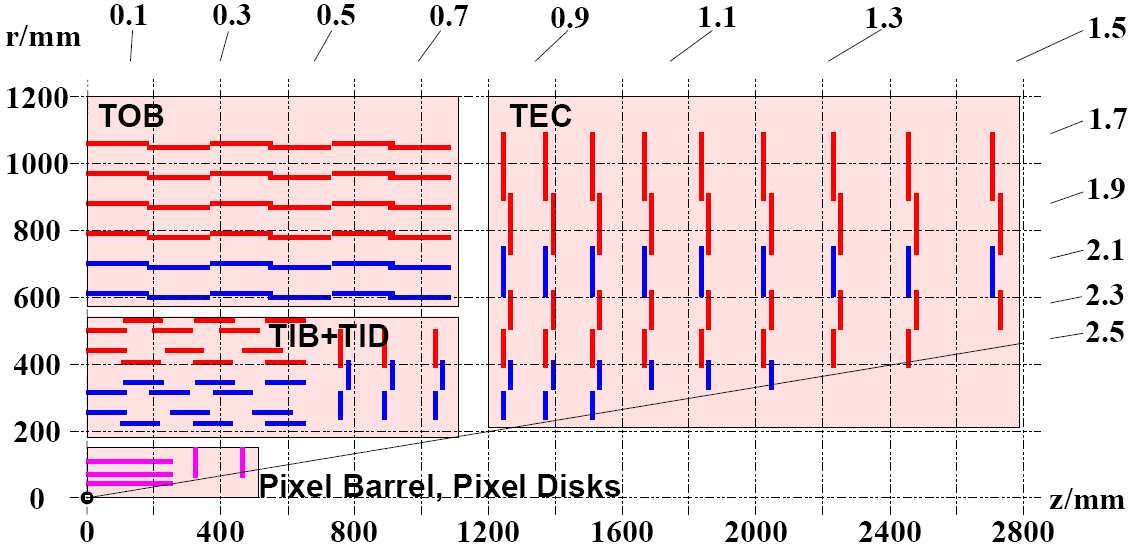
\includegraphics[width=\textwidth]{figures/TrackerLayout.png}
    \caption[
      dasdas
    ]{
    A quarter view of the CMS tracker. The blue lines represent strips sets of two strips that are slightly off parallel from each other.
    }
    \label{fig:trackerLayout}
    
\end{figure}


\subsection{Electromagnetic Calorimeter}
The Electromagnetic Calorimeter(ECAL) is located directly outside of the tracker. It is made of lead tungstate ($\leadtungstate$) scintillating crystals. When an electron or a photon enters a scintillator they create a shower of particles, through processes of bremsstrahlung and pair production. These particles ionize atoms that make up the crystal, which in turn emit photons. By counting the number of photons produced the energy that was deposited in the crystal can be calculated.  Electrons and photons that make it to ECAL deposit almost all their energy into the crystals, allowing the subdetector to accurately measure their energy. However, used by itself, it is difficult to differentiate between the two. To resolve the ambiguity, the tracker is used since electrons, unlike photons, leave a track. 

ECAL was created with the specification that it would be able to detect and accurately measure H$\rightarrow\gamma\gamma$, which set a tight requirement on the energy resolution. The other requirements on ECAL come from the size of the solenoid, which ECAL must fit inside, as well as the high radiation environment. The closely-spaced bunches of the LHC require the ECAL to have a fast response ($<$\SI{25}{\nano\second}). Lead tungstate crystals fulfill these requirements, having a radiation length of $X_0= \SI{0.89}{\centi\meter}$ which allows the crystals to be short while having both the particles deposit most of their energy with a length of $\approx25X_0$, and a Moliere radius of 2$\SI{2.2}{\centi\meter}$, which allows for high granularity and a smaller chance of multiple particles shower into the same crystal even at higher luminosities. $\leadtungstate$ produces 80\% of its light in \SI{25}{\nano\second}, with the trade off of only producing 20 photons/MeV.
	
    ECAL is made up of two main parts, the Electromagnetic Calorimeter Barrel , and the Electromagnetic Calorimeter Endcap as  shown in Fig \ref{fig:ecalLayout}. The Electromagnetic Calorimeter Barrel covers the pseuodorapidity range $\eta<1.479$. In order to measure the light produced by scintillation it uses avalanche photodiodes. The Electromagnetic Calorimeter Endcap covers the range $1.479<|\eta|<3.0$ and uses vacuum phototriodes. Both of these are sections created with crystals that are aimed almost directly at the interaction point. They have a slight tilt so that photons do not travel in the gap between crystals and become lost. 
    
\begin{figure}[!htbp]
    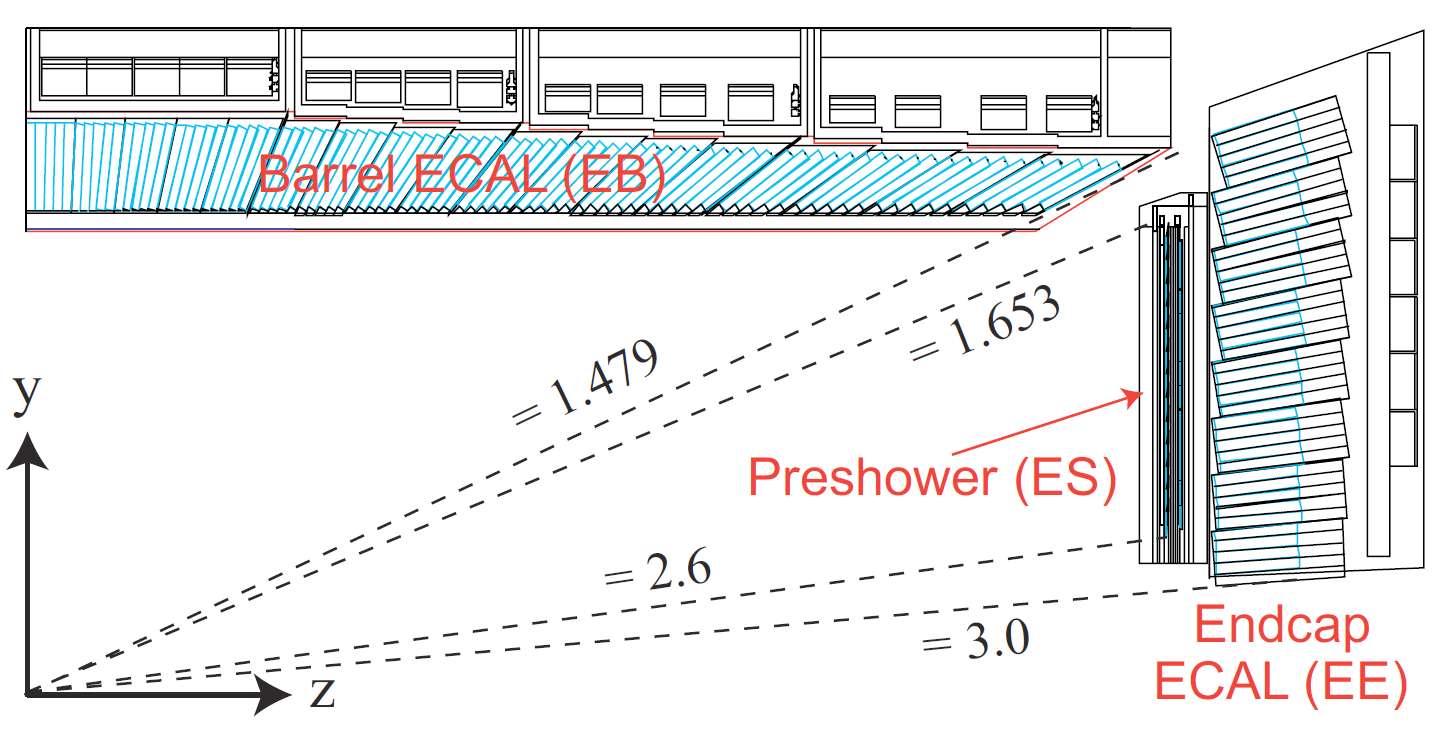
\includegraphics[width=\textwidth]{figures/ecal_layout.png}
    \caption[
      ECAL layout 
    ]{The layout of the Electron Calorimeters of CMS, showing the relationship of the barrel and endcap subdetectors. 
}
    \label{fig:ecalLayout}
    
\end{figure}


\subsection{Hadron Calorimeter}
\begin{figure}[!htbp]
    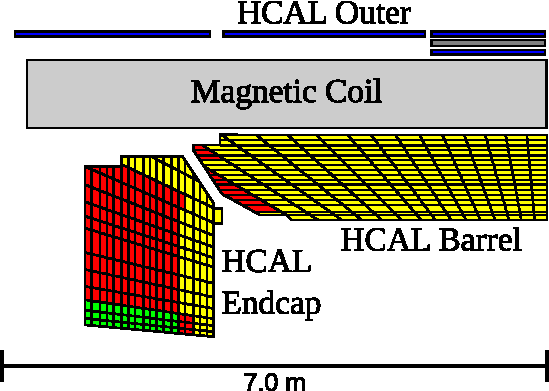
\includegraphics[width=\textwidth]{figures/hcal_cross_section.pdf}
    \caption[
      HCAL layout
    ]{
    The Hadron Calorimeter layout of CMS. It lies directly outside of ECAL, and, therefore, only measures hadrons as well as the rare muon.
    }
    \label{fig:hcalLayout}
    
\end{figure}

The Hadron Calorimeter(HCAL), whose layout is shown in Fig. \ref{fig:hcalLayout}, is built around ECAL and was created to measure the energy of hadrons. HCAL was built with three major requirements.  HCAL was required to be compact so that it could fit inside the solenoid, as well as being cheap, since the lead tungstate crystals that made up ECAL were so expensive. The last requirement was to accurately measure $E^{miss}_T$, which requires good energy resolution, as well as having no gaps that energy could be lost in. This is vital to finding the energy of non-interacting particles, such as neutrinos, as well as other non-standard model particles such as dark matter. In order accomplish these tasks, HCAL was constructed as a sampling calorimeter. The barrel and endcap, Hadron Barrel and Hadron Endcap respectively, of HCAL cover the pseudorapidity range $|\eta|<3.0$. They are made of alternating layers of absorbers and scintillators. The absorber is made of brass, which was chosen due to its being non-magnetic, having a short interaction length, and low cost. The measurements of the energy are done with plastic scintillators that are sandwiched between the layers of absorbers. The light created by the scintillation is transported to hybrid photodiodes by way of wavelength-shifting fibers. 

The Hadron Outer Calorimeter, exists as a single layer outside of the solenoid. Because hadrons have such a large interaction length, some of the hadrons are not completely stopped by the end of HCAL, and can even go through the solenoid. This is more common at very low pseudorapidity since this region  has the least amount of material to transverse.  The Hadron Outer Calorimeter then can help catch the tail end of these showers.

The forward calorimeter covers the pseudorapidity range $3<|\eta|<5$.  The high rapidity range means that this sub detector receives a higher rate of radiation, which requires it to be more radiation hard then the rest of HCAL. It is made out of a bulk steel absorber with quartz fibers running through it pointed towards the interaction point. These quartz fibers do not scintillate; instead, the calorimeter detects Cherenkov radiation that charged particles emit when traveling through the quartz fibers. There are two different types of these fibers - short and long, with the long fibers capable of detecting particles throughout the entire sub-detector while the short fibers start \SI{22}{\centi\meter} from the inner face of the steel absorber allowing for information of the depth of the shower to be measured. 


\subsection{Muon Chambers}
The muon chambers surround the rest of the detector, including the solenoid itself. At this position almost all other observable particles produced have been absorbed, making the identification of muons much easier. The muon system  measures muons' energy similar to the tracker, in that it measures the curve of the muon in the magnetic field. However, since the muon chambers cover a much larger volume than the tracker, it is not practical to use the same silicon sensors. Instead, gaseous detectors are used. These come in three types: drift tube chambers, resistive plate chambers, and cathode strip chambers.
\subsubsection{Drift Tube Chambers}
The drift tube chambers are used in the barrel region of the muon chamber, which covers the range of $|\eta|<1.2$. They consist of a gas filled tube with a wire strung through the center that is kept at a high positive voltage.  When a muon travels through the chamber it ionizes the gas, leading to an avalanche of electrons to deposit charge on the wire. By measuring the timing of when this signal reaches both ends of the wire it is possible to calculate the position of the muon.

\subsubsection{Resistive Plate Chambers}
The resistive plate chambers are made of charged parallel plates that cover $|\eta|<2.1$. The positively charged plate is separated into strips, so that when an avalanche is created the muon's position can be measured. The resistive plate chambers have a worse position resolution then the drift tube chambers but a better timing measurement, aiding in crosschecks in the barrel region. 

\subsubsection{Cathode Strip Chambers}
The Cathode Strip Chambers are used in the endcap, which covers $1.2<|\eta|<2.4$. Rather then having a single anode in each chamber as the Drift Tubes does, it is made up of chambers with positively charged wires and negatively charged copper strips, with the strips parallel to the radial direction, and the wires parallel to the $\phi$ direction. The electron avalanche deposits charge on a wire giving a radial measurement, while an image charge forms over multiple strips allowing for an accurate $\phi$ measurement to be made.  This is done due to the higher $\eta$, which leads to higher background levels, as well as a less uniform magnetic field, both of which require more precise measurements. 

%%%%%%%%%%%%%%%%%%%%%%%%%%%%%%%%%%%%%%%%%%%%%%%%%%%%%%%%%%%%%%%%%%%%%%%%%%%%%%%%
\section{Data Storage and Triggering}
Although creating a detector that is capable of working with the speed and accuracy required while being radiation hard was perhaps the most obvious engineering issue in the creation of CMS, it was in no way the only one. Another obstacle is the sheer scale of the data produced. In 2012, bunches collided every  \SI{50}{\nano\second}. Therefore it is impractical to save every event. Fortunately it is also not necessary, because the vast majority of events do not contain interesting interactions and do not need to be saved. Consider Fig \ref{fig:Rates}, which shows the cross-sections (or rates) for a range of processes at the LHC. While the soft collisions may occur at nearly one GHz, interesting events such as Z boson occur at a few tens of Hz and \higgstogammagamma at less than one per a hour.
\subsection{Pileup and QCD Background}
\label{Sec:Pileup}
One of the important factors in triggering and data volume is pileup. Pileup occurs when multiple interactions happen in the same event. Because of the strength of the strong force, the vast majority of pileup events are QCD interactions. For each bunch crossing roughly 20 sets of protons interact, leading to large sprays of hadrons, the majority being pions. This pileup complicates measurements since it tends to deposit energy in multiple different parts of both HCAL and ECAL that must be compensated for. 
A second issue comes from jets produced from non-interesting interactions. As can be seen from Fig \ref{fig:Rates}, jets, while not produced in every event, are still produced in a large enough fraction of events that it is difficult to have the trigger save events based on jets such as \Wtoqq, due to the high rate of QCD-based jets. 
\subsection{Trigger}
\label{Sec:Trigger}
\begin{figure}[!htbp]
    \centering
    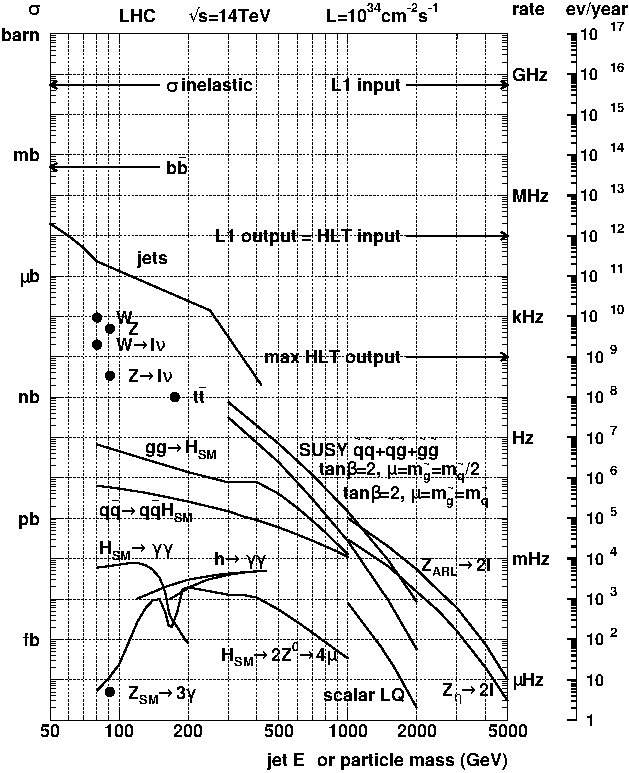
\includegraphics{figures/ExperimentFigures/rates_lhc.pdf}
    \caption[Cross sections in the LHC]{This shows the relative cross sections as well as rates for multiple different interactions in CMS. Theoretical particles cross sections are shown as a a function of their mass.}
    \label{fig:Rates}
\end{figure}
Although beam crossing at the LHC happens at a rate of 40 MHz, data itself is only saved at, on average, a rate of around 400Hz. In order to decide which events to save, a two-stage trigger is used. The first stage, called the Level 1 trigger removes 99.75\% of events, lowering the rate to 100KHz. It does this through customized hardware. Because the L1 trigger is required to make decisions at a high rate to keep up with bunch crossings, this hardware must be very quick. In order to accomplish this, the trigger looks at a very simplified version of the CMS detector. For example it does not look at individual crystals of ECAL but clusters of them, as well as not looking at the depth information from HCAL. 

The second trigger system is known as the High Level Trigger. Because the High Level Trigger only receives 0.25\% of the events the L1 trigger receives, it can spend over 100 times longer making decisions, allowing it to use  more sophisticated methods. This increase in time allows the High Level Trigger to make decisions based on the detector as a whole, as well as use more complex algorithms to make the decision. An example would be when attempting to trigger on electrons, the High Level Trigger could look for a charged track in the tracker that leads to a deposit of energy in ECAL, with little energy deposited in the corresponding section of HCAL. In order to be able to accomplish these tasks, the High Level Trigger uses much software than the L1 trigger, and uses more standard computer hardware. The High Level Trigger is able to remove 99.6\% of bunch crossings that pass the L1 trigger. 





\section{Electron Reconstruction} 
The process of reconstructing the energy and momentum of an electron is an excellent example of the complementarity of the CMS subdetectors. At the limit of very low energy, the electron path is highly curved, allowing the tracker to very accurately measure its momentum, whereas at high energies the path becomes so straight that it is hard to measure its energy using the tracker. However at high energies ECAL becomes more accurate. By comparing the measurements of both the tracker and ECAL, particles can be measured over a wide range of different energies.

The two subdetectors also allow for the rejection of other charged particles, such as pions. This is done by comparing the energy measured by the tracker to the energy deposited by the particle into ECAL. Since pions tend to not deposit all their energy into ECAL, a mismatch between the two subdetectors is a sign that the particle is not an electron. This can also be used to remove photons, since they leave no track at all, so a crystal that has energy deposited in it with no corresponding track would be reconstructed as a photon. Even photons who happen to line up with a track can be rejected if the track's energy does not match the energy deposited in the crystal.

In practice, the energy deposited in a single crystal of ECAL can not be directly compared to the energy of a track since the passage of an electron through the CMS tracker often involves significant scattering and emission of bremsstrahlung photons. These photons are not affected by the magnetic field of the detector so they travel in a straight line unlike the electron. When the electron does hit a crystal, the shower it creates bleeds into other crystals. In order to reconstruct the original energy of the electron, it is necessary to include these energies by measuring the energy deposited in a cluster of crystals near the central crystal. Super-clusters are then created to take into account the photons that were emitted due to Bremsstrahlung radiation. Because the magnetic field causes the electron to bend primarily in the  $\phi$ direction, the super-clusters are not circularly symmetric, but extend further in the $\phi$ direction than in $\eta$. The super-cluster is then matched to a track from the tracker. The algorithm constructs an electron track using a “Gaussian Sum Filter” (GSF)\cite{adam_2005}. This is a modified version of the standard Kalman filter used for muons and hadrons, and was created to handle the large energy loss and corresponding large change in path of the electron when traveling through the tracker. The final $\eta$ and $\phi$ measurement for electrons uses data from the tracker, while the energy measurement optimally combines ECAL and tracker measurements as a function of energy, putting more weight on ECAL as the momentum rises.
 \subsection{Corrections to the Electron}
 In order to increase the accuracy of the reconstructed electron, two sets of corrections are applied to the data as well as the reconstructed electrons in the simulation. These corrections affect the reconstructed momentum of the electrons. In general, the impact of these corrections is limited for the analysis described here, as the angle measurement of the lepton is more critical than the energy. However, because the acceptance sets a requirement on energy, the energy corrections do have some effect. 
 \subsection{Regression}
 In order to improve the reconstructed energy of ECAL, a regression was used. This is necessary since the measurement of energy in the ECAL is affected by a large number of additional effects, primarily the loss of a portion of the energy of the electron in cracks and dead materials. It is difficult to write an analytic correction for these effects but they are well represented by the simulation of CMS. To provide a correction, we categorize aspects such as shower shape, and the location in ECAL, as well as 39 other variables in an  automated technique through a boosted decision tree. This is trained on $\Ztoee$ and $\higgstoZZ$ simulation\cite{cms_an_2012-327}.  The regression was trained separately for both the Electron Barrel and Electron Endcap. Half of the sample was used to train the regression, while the other half was used for validation. Electrons used are required to have $\pt>\SI{7}{GeV}$, as well as have emitted less than 1\% of its initial energy in the form of FSR. An example showing the effects of this regression are shown in Fig. \ref{fig:regression example}. This example was picked due to how visibly the regression improved the measured value of the electron's energy. The reason for the vast improvement is this region includes electrons that are near the separation between the barrel and the endcap of ECAL, which exaggerates the impact compared with more uniform regions of the detector.
\begin{figure}[!htbp]
    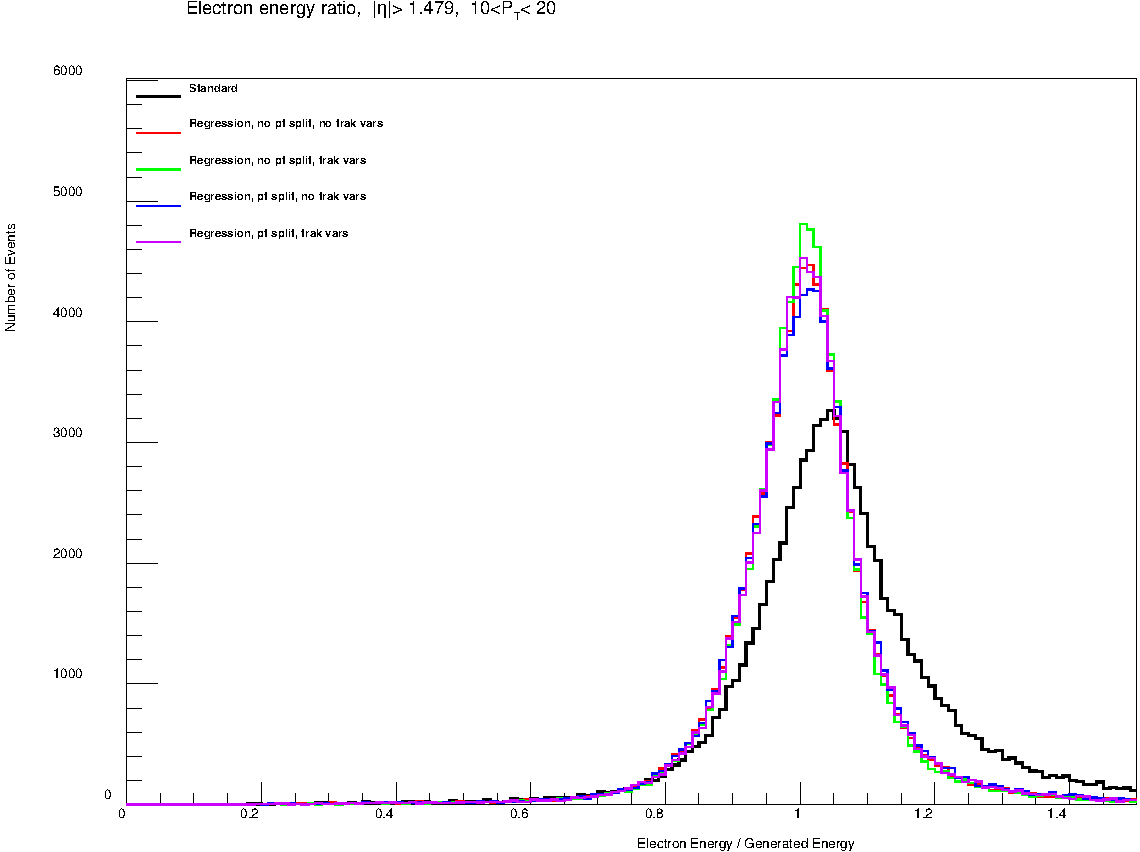
\includegraphics[width=\textwidth]{figures/ExperimentFigures/ExampleRegressionCropped.pdf}
     \caption{An example showing the effects of the regression method on a specific subset of electrons. The ratio of generated energy of an electron to the reconstructed energy is on average closer to one after the regression}
     \label{fig:regression example}
 \end{figure}
 \subsection{Energy Scale and Resolution}
 Energy scale and resolution effects were further corrected using two methods based on a $\Ztoee$ sample\cite{cms_an_2013-253}. The purpose of this was to create better agreement between the simulation and the data for parts in which the simulation less accurately represents the detector.
 
 In the first method, the data and simulations were fit with a convolution of a Breit-Wigner with a Crystal Ball function. The Crystal Ball function gets its name from an early spherical crystal calorimeter and the collaboration which developed the function to reproduce the characteristic response of a segmented total absorption calorimeter\cite{oreglia_1980}.  The Crystal Ball function is a power-law below a threshold value, and a Gaussian above the threshold. The Crystal Ball is used for modeling the detector resolution as well as losses in the tracker due to the bremsstrahlung. The Breit-Wigner distribution is used to model the resonance of the \Z itself, and uses the nominal values from the Particle Data Group with a nominal mass of $\MZ=\Zmass$ and a width of $\GammaZ=\Zwidth$. Because the state of the detector changes over time, there is a time dependence of the scale correction, as well as an inherent pseudorapidity dependence. The fit was done for four different pseudorapidity bins as well as various run ranges. The scale correction, $\Delta P$, was then taken to be the difference between the peak of the Crystal Ball function of both data and signal and is calculated using  
 \begin{equation}\label{eq:ScaleCor}
     \Delta P
     =
     \frac{\Delta m_{\text{Data}} - \Delta m_{\text{MC}}}{\MZ}.
 \end{equation}
 
 
 The second method further separates electrons based on the parameter $R_9$. This variable is defined as the energy in the 3$\times$3 set of crystals around the peak of the shower over the super-cluster as a whole. Therefore, larger showers give smaller $R_9$ values.  Showering electrons are defined as $R_9<0.94$, and non-showering are defined as $R_9>0.94$. A probability distribution function of the mass of the Z based on simulation is created in which the energy of each super-cluster in the simulation is multiplied by a Gaussian factor centered at $\Delta P$ with a standard deviation of $\Delta\sigma$. The $\Delta\sigma$ is calculated separately for both types of electrons, the four rapidity bins, and the different runs using likelihood maximization.  In electron barrel, due to a large amount of statistics, it was also possible to further subdivide in terms of $\ET$, allowing for corrections to be created based on $\ET$.
 
